\section{Design of \sys}
\label{s:impl}

\sys is a coverage-directed concurrency fuzzer to effectively discover
concurrency bugs.
%
The key improvement of \sys lies in adopting interleaving segment
coverage and the coverage-directed interleaving \dr{}mutation
algorithgm described in \autoref{s:design}.
%

\dr{TODO: why do we explain instrumentation and engine first, fuzzer
  later}


In the following of subsections, we describe design details of the
target kernel instrumentation~(\autoref{ss:instrumentation}) and the
execution engine~(\autoref{ss:engine}), followed by the userspace
fuzzer~(\autoref{ss:fuzzer}).  Lastly, we explain the implementation
details of \sys~(\autoref{ss:impl}).


\subsection{Target Kernel Instrumentation}
\label{ss:instrumentation}

\sys requires to profile basic blocks and memory accesses executed by
each system calls.
%
To this end, \sys incorporates a compiler pass that inserts callback
function calls 1) at the beginning of each basic block, and 2) before
each instruction that accesses globally-visible memory objects.
%
These callback functions trace basic blocks and memory accesses during
the execution in the kernel, and records them into memory regions
shared between the user space and the kernel space.



\begin{figure}
  \centering
  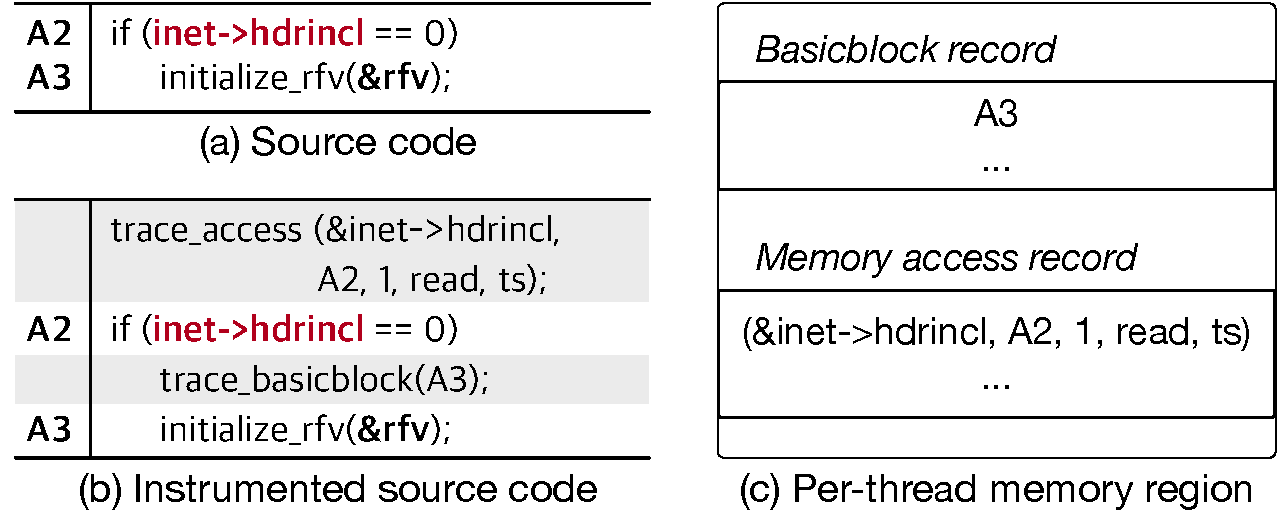
\includegraphics[width=\linewidth]{fig/instrumentation.pdf}
  \caption{(a) A part of \texttt{raw_sendmsg()} in
    \autoref{fig:cve-2017-17712}, (b) abstract of the intrumented
    binary, and (c) memory accesses and basic blocks recorded during
    runtime.}
  \label{fig:instrumentation}
\end{figure}

\autoref{fig:instrumentation} shows how the \sys's compiler pass
inserts callbacks, and how each callback records memory accesses and
basic blocks.
%
When compiling a source code in (a), the compiler pass inserts
function calls \texttt{trace_basicblock()} at \texttt{0x0} (\ie, the
beginning of the compiled function) and \texttt{0x12} (\ie, the
beginning of the basic block).
%
Similarly, the compiler pass inserts a function call
\texttt{trace_access()} at \texttt{0x5}, which is right before an
instruction that accesses \texttt{inet->hdrincl} at \texttt{0xa}.


During runtime, \texttt{trace_basicblock()} takes the instruction
address of the function call as input (\ie \texttt{0x0} and
\texttt{0x12}), and records the instruction address into
\texttt{Basicblock record}.
%
On the other hand, \texttt{trace_access()} takes four parameters, the
address of the accessed memory object (\ie, \texttt{\&inet->hdrincl}),
the instruction address accessing the memory object (\ie,
\texttt{0x5}), the size of the memory access (\ie, \texttt{1}), and
the type of the memory access (\ie, \texttt{read}), and records them
into \texttt{Memory access record}.






It is worth noting that \texttt{Basicblock record} and \texttt{Memory
  access record} are per-thread memory regions, which is shared
between the user space and the kernel space. Thus, after threads of
the userspace fuzzer execute system calls, each thread can identify
basic blocks and memory accesses executed by a system call that it
executed.









% Unlike data race detectors such as KCSAN~\cite{kcsan}, the \sys's
% scheduling mechanism needs to recognize both plane memory accesses and
% annotated memory accesses such as atomic operations.
% %
% We deal with these two types of accesses differently since annotated
% accesses usually are implemented in assembly code, which is hard for a
% LLVM pass to understand.
% %
% In order to instrument plane accesses, we implement a LLVM pass that
% insert callback function calls after memory accesses on LLVM IR.
% %
% Our pass runs after most of binary transfomration is done, so it
% \XXX{...}.
% %
% For annotated instructions, we rely on the functionality of
% KASAN~\cite{kasan} to instrument atomic operations.
% %
% KASAN provides wrapper functions of annotation APIs to call callback
% functions before annotated memory operations, and we instruct the
% wrapper functions to call our callbacks as well.
% %
% Our callbcak functions write memory access operations along with
% various information into a region mmap-ed shared region shared by a
% userspace program (\ie, fuzzer) and a kernel. The information about
% memory operations includes the instruction address, the start address
% of a memory location, and the size of memory access.
% %
% Accordingly, a fuzzer is able to identify what memory access
% operations took place during the execution.

% \sys also requires an additional module called a trampoline that is
% used to suspend and resume a running thread. Details about the
% trampoline are described in \autoref{ss:engine}.


\subsection{Execution Engine}
\label{ss:engine}

In order to allow the userspace fuzzer to control thread scheduling,
\sys introduces an execution engine.
%
The execution engine is implemented in the hypervisor layer to be
non-intrusive to the kernel execution, the userspace fuzzer requests
the execution engine to control thread scheduling through hypercall
interfaces.

\PP{Schedule}
%
A schedule is a specification of how to control thread scheduling.
%
It contains per-system call sequences of scheduling points, where each
scheduling point is described as a two-tuple, (instruction address,
scheduling order).

\begin{figure}[t]
  \centering
  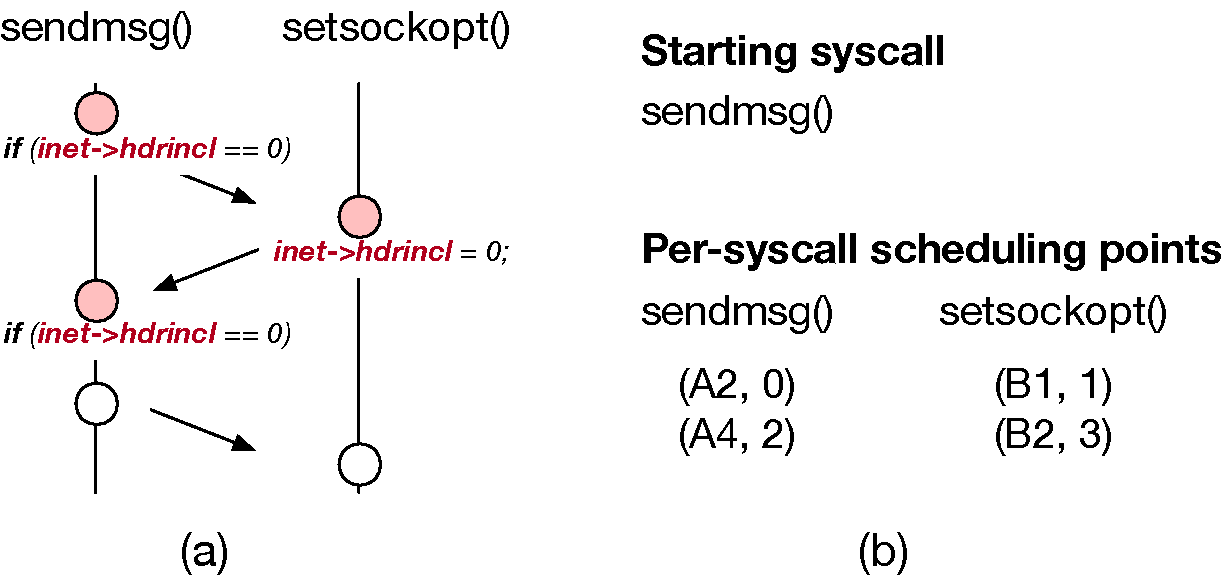
\includegraphics[width=0.9\linewidth]{fig/schedule.pdf}
  \caption{(a) Thread interleaving to run, and (b) Schedule specifies
    scheduling points for (a).}
  \label{fig:schedule}
\end{figure}

\autoref{fig:schedule} illustrates an example of a schedule. In order
to run a thread interleaving in \autoref{fig:schedule}-(a), four
preemptions are required at \texttt{A2}, \texttt{B1}, \texttt{A6}, and
\texttt{B2}.
%
And each schedule point denotes on which these preemptions occur,
annotated with the order of preemption.


During fuzzing, the userspace fuzzer keeps generating different
schedules, and requests the execution engine through hypercall
interfaces to control thread scheduling according to a schedule.





\PP{Thread scheduling control}
%
Through hypercall interfaces, the execution engine accepts a schedule
from the userspace fuzzer. After that, when threads of the userspace
fuzzer execute sytsem calls, the execution engine controls thread
scheduling as described in the given schedule.

%
\begin{figure}[t]
  \centering
  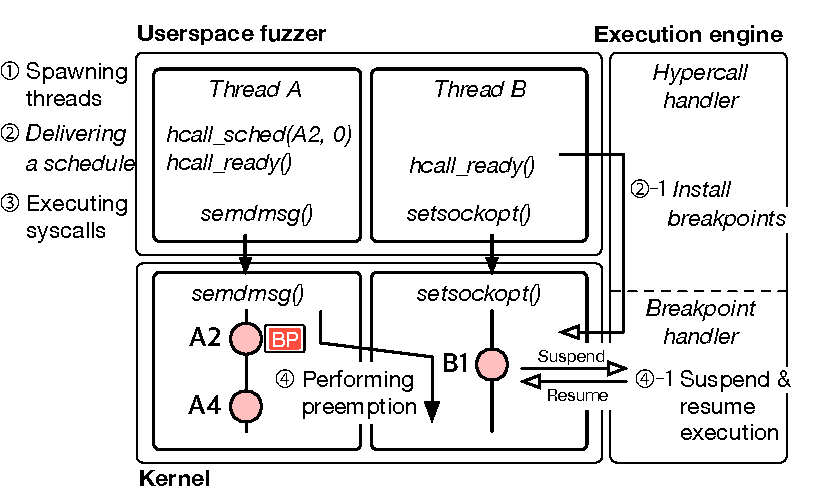
\includegraphics[width=0.9\linewidth]{fig/workflow-hypervisor.pdf}
  \caption{The workflow of the execution engine. \red{IMPORTANT: this
      is copied from AITIA. Need to redraw}}
  \label{fig:workflow-hypervisor}
\end{figure}
%
\autoref{fig:workflow-hypervisor} shows a workflow of the execution
engine.
%
At the beginning, the userspace fuzzer spawns threads that are
responsible to execute system calls concurrently.
%
Then, each thread is assigned a system call and its scheduling points.
\dr{}


each thread calls hypercalls to deliver scheduling points to
the execution engine before executing a system call.



After the fuzzer sends a schedule, the userspace fuzzer notifies the
execution engine, and the execution engine starts executing with the
intial thread specified in the given schedule while other threads are
suspended.

%
When the running thread reaches a scheduling point, a hypervisor
performs preemption by suspending the running thread and resuming the
next thread to run in order to enforce the execution order between
memory access operations.
%
\dr{TODO:}
Details about suspending and resuming a thread is described later.


\PP{Suspending a thread}
%
A few prior approaches~\cite{ski, snowboard, razzer} suspend a vCPU
instead of a guest thread. While suspending a vCPU grants the ability
to control an interleaving, it is not suitable for our purpose because
suspending a vCPU may unexpectedly suspend another vCPU. An example we
observed is TLB shootdown~\cite{tlbshootdown}. When a vCPU wants TLB
shootdown, it sends inter-process interrupts (IPIs) to all cores and
wait until all cores to execute the TLB shootdown handler.  In this
case, if one vCPU is entirely suspended, the TLB shootdown cannot be
successfully conducted causing the vCPU invoking TLB shootdown
blocked.
%
Therefore, instead of adopting the prior approach, our hypervisor is
designed to suspends and resumes a guest thread.
%
In order to suspend a thread at an arbirary location, we use a
hardware breakpoint functionality~\cite{hwbp} shipped in modern Intel
CPU chipsets.
%
When a guest thread hits a breakpoint, our hypervisor saves its
register values and then changes the program counter of the thread to
an infinite loop called trampoline. In the trampoline, the thread
keeps calling \texttt{cond_resched()} to yield a CPU to make all other
kernel functionalities (\eg, handling the TLB shootdown handler) work
normally. When the guest thread resumes, our hypervisor restores
registers with the values saved when the thread is suspended, and the
thread continues its execution.


\PP{Virtual Machine Instrospection}
%
While controlling thread scheduling of system calls, the execution
engine introspects the target kernel for two reasons.
%
First, because a hardware breakpoint does not distinguish which thread
hit the breakpoint, it needs to determine whether the breakpoint is
hit by a thread of the userspace fuzzer, when a breakpoint is hit.
%
If it is the case, the execution engine suspends the running thread
and resumes the suspended thread as specified in a schedule.
%
Otherwise, the execution engine ignores the breakpoint hit, and keeps
running the kernel.


%
Second, when a running thread tries to acquire a lock, the execution
engine need to inspect the lock is held by a suspended thread to
prevent a situation 
%
If a running thread is trying to acquire a lock, the execution engine 



While the virtual machine introspection is crucial to properly control
thread scheduling, we leave details of the virtual machine
introspection in \autoref{s:appendix:vmi}.



\subsection{Userspace Fuzzer}
\label{ss:fuzzer}



\begin{figure}
  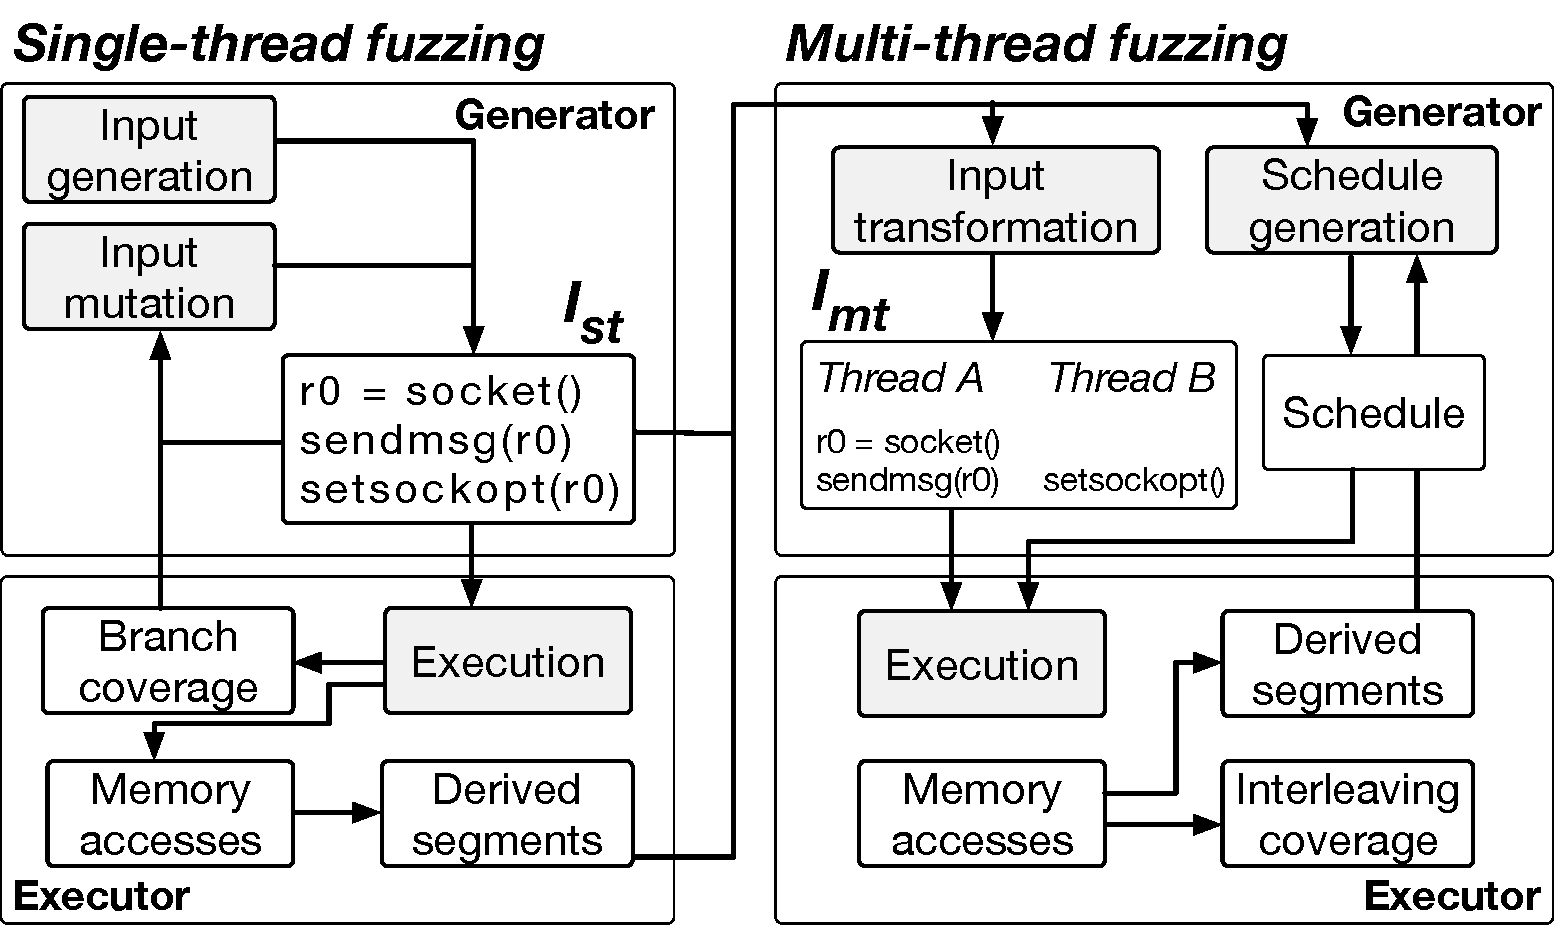
\includegraphics[width=0.9\linewidth]{fig/architecture.pdf}
  \caption{Workflow of \sys \dr{TODO: redraw to describe the workflow}}
  \label{fig:workflow}
\end{figure}


The \sys's userspace fuzzer conducts two-stage pipelined fuzzing
similar with recent concurrency fuzzers, Razzer~\cite{razzer} and
Snowboard~\cite{snowboard}.
%
In \sys, the first stage is a \textit{single-thread} fuzzing that
focuses on expanding code coverage, and the second stage is a
\textit{multi-thread} fuzzing to explore thread interleavings.

Both stages consists of two components, an input generator and an
input executor. We explain details of each component in the following.


\subsubsection{Single-thread fuzzing}
%
In a single-thread fuzzing phase, the single-thread generator
generates a single-thread input (refered as $I_{ST}$) in the form of a
sequence of random system calls.
%
And then, the single-thread executor executes $I_{ST}$ to perform two
things.
%
First, it collects code coverage of $I_{ST}$ with the purpose of
exploring source codes residing deep inside the kernel.
%
Second, it identifies two system calls in $I_{ST}$ that potentially
exhibit new interleaving coverage.  If identified, $I_{ST}$ will be
handed to the next phase, namely the multi-thread fuzzing.


\PP{Single-Thread Generator}
%
The single-thread generator is similar with conventional
fuzzing~\cite{syzkaller}.
%
It constructs a single-threaded system call sequence $I_{ST}$ with two
strategies: generation and mutation.
%
When using the generation strategy, \sys randomly generates a system
call sequence based on well-formed system call description grammar
\texttt{Syzlang}~\cite{syzlang}.
%
\texttt{Syzlang} describes templates of available system calls
including types of arguments and the type of a return value, as well
as a range of feasible values of each arguments.
%
According to \texttt{Syzlang}, \sys produces a single-thread system
call sequence by repeatedly selecting a random system call and
providing reasonable arguments of the system call.

The mutation strategy is an alternative of the generating strategy.
When using a mutation strategy, \sys picks up a already-generated
single-thread input, and modifies the single-thread input by appending
additional system calls, removing existing system calls, or changing
values of arguments of existing system calls.


\PP{Single-Thread Executor}
%
Given $I_{ST}$ from the single-thread generator, the single-thread
executor runs $I_{ST}$, and profiles basic blocks and memory accesses
executed by each system call with a support from instrumentation
detailed in \autoref{ss:instrumentation}.

With profiled basic blocks and memory accesses, the single-thread
executor conducts two tasks.
%
The first task is similar with what conventional kernel fuzzing
does.
%
In other words, the single-thread executor computes branch coverage
using profiled basic blocks.
%
Then, if $I_{ST}$ exposes new branch coverage that has not been
explored, \sys keeps $I_{ST}$, and feeds it back to the single-thread
generator so that the single-thread generator further mutates $I_{ST}$
to find more branch coverage.
%
As a result, \sys keeps a minimal set of $I_{ST}$, called a corpus,
which may execute previously-executed branches when running
single-thread inputs in the corpus.


Second, the single-thread executor identifies a pair of system calls
in $I_{ST}$ potentially exposes new interleaving coverage if executed
concurrently.
%
More specifically, for each pair of system calls, the single-thread
executor checks  \dr{}
%



\subsubsection{Multi-thread fuzzing}
%
After $I_{ST}$ is handed with a pair of system calls to execute
concurrently, the multi-thread generator transforms $I_{ST}$ to a
multi-thread input $I_{MT}$.
%
In addition, the multi-thread generator generates \textit{schedules}
where each schedule describes how to enforce thread interleaving (\ie,
a set of scheduling points) during runtime.


The multi-thread executor then repeatedly tests each schedule of
$I_{MT}$ one at a time.
%
To this end, the multi-thread executor instruments $I_{MT}$ with
hypercalls in order to tell the execution engine how to control thread
scheduling.
%
Lastly, the multi-thread executor runs $I_{MT}$ while enforcing a
given schedule with a support of the execution
engine~(\autoref{ss:engine}).




\PP{Multi-Thread Generator}
%
% In order to use interleaving graph as interleaving coverage, we need a
% method to store them, and compare them to a new interleaving graph.
% %
% We choose to use a hash value of

% the FNV-1~\cite{fnv, fnv-go}, non-cryptographic hash function,


% A schedule is an outcome of the interleaving mutation.
% A schedule contains an initial thread, and a set of scheduling points
% indicating an instruction on which preemption occurs.


With a given $I_{ST}$ and a pair of system calls, the multi-thread
generator transforms it to $I_{MT}$.




\PP{Multi-Thread Executor}
%
A 





\subsection{Implementation}
\label{ss:impl}

We implement \sys in various software layers.
%

%
To allow 


We use scc~\cite{scc} and sloccount~\cite{sloccount} to measure LoC of
GO and C respectively.


%%% Local Variables:
%%% mode: latex
%%% TeX-master: "p"
%%% End:
